\documentclass[11pt,a4paper]{ctexart}
\usepackage[a4paper,margin=1.75cm,headheight=15pt]{geometry}
\usepackage{amsmath,amssymb,mathtools,booktabs,tabularx,array,enumitem}
\usepackage[most]{tcolorbox}
\usepackage{tikz}
\usetikzlibrary{arrows.meta,positioning,calc,fit}
\usepackage{xcolor,fancyhdr,hyperref,microtype,lastpage}
\newcolumntype{Y}{>{\raggedright\arraybackslash}X}
\newcolumntype{L}[1]{>{\raggedright\arraybackslash}p{#1}}
\newcolumntype{C}[1]{>{\centering\arraybackslash}p{#1}}
\setlength{\parindent}{2em}
\setlength{\parskip}{0.34em}
\setlength{\emergencystretch}{3em}
\renewcommand{\arraystretch}{1.2}
\setlength{\tabcolsep}{3pt}
\setlist[itemize]{itemsep=0.18em,topsep=0.35em,leftmargin=2em}
\setlist[enumerate]{itemsep=0.18em,topsep=0.35em,leftmargin=2em}
\definecolor{deep}{RGB}{35,64,76}
\definecolor{soft}{RGB}{244,247,247}
\definecolor{greenish}{RGB}{49,91,73}
\definecolor{warnc}{RGB}{137,61,55}
\definecolor{purple}{RGB}{82,72,112}
\definecolor{rulegray}{RGB}{108,114,118}
\hypersetup{colorlinks=true,linkcolor=deep,urlcolor=purple,pdftitle={NET-05 路由与控制平面}}
\pagestyle{fancy}
\fancyhf{}
\lhead{\small\color{deep}\textbf{408 · 计算机网络 NET-05}}
\rhead{\small\color{deep}Knowledge · Policy · Convergence · Install}
\cfoot{\small 第 \thepage\ 页 / 共 \pageref{LastPage} 页}
\renewcommand{\headrulewidth}{0.4pt}
\newtcolorbox{corebox}[1]{breakable,colback=soft,colframe=deep,title=\textbf{#1},boxrule=0.8pt,arc=2mm}
\newtcolorbox{methodbox}[1]{breakable,colback=white,colframe=greenish,title=\textbf{#1},boxrule=0.7pt,arc=1.5mm}
\newtcolorbox{warnbox}[1]{breakable,colback=white,colframe=warnc,title=\textbf{#1},boxrule=0.7pt,arc=1.5mm}
\newtcolorbox{examplebox}[1]{breakable,colback=white,colframe=purple,title=\textbf{#1},boxrule=0.7pt,arc=1.5mm}
\newcommand{\kw}[1]{\textbf{\color{deep}#1}}
\newcommand{\code}[1]{\texttt{#1}}
\tikzset{net/.style={draw=deep,rounded corners=1.5mm,text width=2.65cm,minimum height=0.95cm,align=center,fill=soft,font=\small,inner sep=3pt},flow/.style={-{Latex[length=2mm]},thick,draw=deep},ref/.style={-{Latex[length=2mm]},dashed,draw=rulegray}}

\title{\vspace{-1.1cm}\textbf{路由与控制平面}\\[0.4em]\large 不完整知识怎样收敛为可用转发状态}
\author{408 · 计算机网络 Topic NET-05}
\date{}

\begin{document}
\maketitle

\begin{corebox}{母问题：每台路由器只看见局部，网络凭什么形成远端可达性？}
路由不是求一次最短路，而是在消息延迟、拓扑变化和管理策略存在时，持续维护一套可供转发使用的分布式知识：
\[
\boxed{\begin{gathered}
\text{Local Observation}\to\text{Advertisement}\to\text{Knowledge Merge}\\
\to\text{Decision under Objective/Policy}\to\text{Install Forwarding State}
\end{gathered}}
\]
箭头表示知识的生成与提交顺序。拓扑一旦变化，这条链会再次运行；传播完成之前，不同节点持有不同版本的世界是正常中间态。
\end{corebox}

\begin{methodbox}{本册定位与 Owner 边界}
\begin{itemize}
  \item \kw{Owns：}DV/LS/path-vector 知识表示，RIP/OSPF/BGP，AS 与 area，RIB candidate/selection，convergence，control/data plane，以及 SDN 的逻辑集中控制模型。
  \item \kw{Uses：}图与最短路算法作为计算工具；NET-04 的 prefix/FIB/LPM 作为转发接口。
  \item \kw{Stops：}当前 packet 如何查 FIB、ARP 下一跳和重封装由 NET-04/NET-02 拥有；本册不把路由写成纯图算法，也不承诺某协议瞬时全局一致。
\end{itemize}
\end{methodbox}

\section{独立阅读词典：路由系统中的每个名词指什么}

\begin{center}
\small
\begin{tabularx}{\linewidth}{L{2.5cm}L{4.1cm}Y}
\toprule
术语 & 本册中的可操作定义 & 不要混成什么 \\
\midrule
router & 读取目的地址并选择下一跳/出口的网络设备 & 不是只负责学习路线的程序 \\
control plane & 产生、比较和安装路线状态的部分 & 不等于当前正在搬运 packet 的路径 \\
data plane & 使用已安装 FIB 对每个 packet 做快速查找和转发的部分 & 不负责理解全网拓扑 \\
distance vector (DV) & 只交换“我到各目的地的距离/代价”这一压缩结论 & 不是完整拓扑图 \\
link state (LS) & 交换“我有哪些邻居链路及其代价”等事实，各节点自行计算 & 不是已经算好的最终路由表 \\
path vector & 通告前缀及经过的 AS 路径和策略属性 & 不是全网统一最短路 \\
AS & 一个由同一管理策略控制、对外作为整体交换路由的自治系统 & 不是一台路由器 \\
metric / policy & metric 是算法用于比较的数值；policy 是管理员定义的取舍规则 & 不能都翻译成“距离” \\
LSDB / SPF & LSDB 是链路状态数据库；SPF 是从数据库算出的最短路径树 & 都不是直接给 packet 查的 FIB \\
convergence & 拓扑变化传播并完成重新计算/安装后，网络状态重新稳定的过程 & 不是瞬间全网同步 \\
\bottomrule
\end{tabularx}
\end{center}

后文的“路线”指“某个目的前缀应从哪个出口/下一跳走”的状态；“路径”指可能经过的
节点序列；“转发”指数据面已经使用这条状态搬运 packet。三个词不能互换。

\tableofcontents
\newpage

\section{全科坐标：这是知识系统，不只是图算法}

路由问题首先要定位四件事：
\[
\boxed{\text{Scope}\to\text{Knowledge Representation}\to\text{State Owner}\to\text{Event/Time}}
\]

\begin{center}
\small
\begin{tabularx}{\linewidth}{L{2.0cm}L{3.0cm}L{3.0cm}Y}
\toprule
作用域 & 知识表示 & 主要 Owner & 时间事件\\
\midrule
邻居/小型域内 & distance vector & 每台 router 的距离候选 & 周期/触发更新、超时\\
OSPF area & link-state facts/LSDB & area 内每台 router & LSA 更新、洪泛、SPF\\
跨 AS & prefix + path attributes & BGP speaker/本地策略 & UPDATE/withdraw、policy\\
SDN domain & logical topology + rules & controller cluster/device & event、计算、规则安装\\
data plane & installed FIB & forwarding device & packet arrival/LPM\\
\bottomrule
\end{tabularx}
\end{center}

算法只回答“给定某份输入，怎样算结论”；路由协议还必须回答输入从哪里来、怎样辨别新旧、怎样传播、谁能信任谁、何时安装、变化期间怎样失败。

\section{控制平面与数据平面：生成状态与使用状态}

\begin{center}
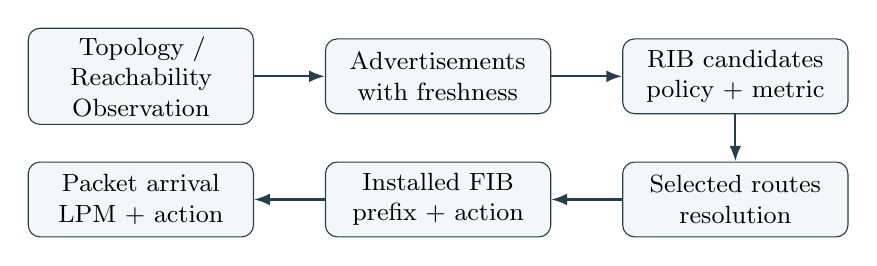
\begin{tikzpicture}[node distance=6mm and 9mm]
\node[net] (obs) {Topology / Reachability\\Observation};
\node[net,right=of obs] (adv) {Advertisements\\with freshness};
\node[net,right=of adv] (rib) {RIB candidates\\policy + metric};
\node[net,below=of rib] (best) {Selected routes\\resolution};
\node[net,left=of best] (fib) {Installed FIB\\prefix + action};
\node[net,left=of fib] (packet) {Packet arrival\\LPM + action};
\draw[flow] (obs)--(adv);
\draw[flow] (adv)--(rib);
\draw[flow] (rib)--(best);
\draw[flow] (best)--(fib);
\draw[flow] (fib)--(packet);
\end{tikzpicture}
\end{center}

RIB 是控制面的候选和选择状态，FIB 是为快速数据面执行安装的状态。具体实现可以合并命名或维护多张表，但解题时必须保留这条语义边界：
\[
\boxed{\text{Route selection}\ne\text{Prefix lookup}}.
\]

\begin{methodbox}{NET-B02 的接口契约}
NET-05 输出 `(destination prefix, selected next hop/interface, action attributes)`；NET-04 接收已安装 FIB，对 destination IP 做 LPM 并执行动作。路由可能收敛而 FIB 尚未完成安装，也可能 FIB 暂时保留旧状态，因此“控制面已算出”不自动等于“此刻 packet 已按新路径转发”。
\end{methodbox}

\section{静态与动态：状态由管理员还是协议更新}

静态路由由管理员直接配置 destination prefix、next hop/egress 与可选 preference，不通过路由协议随拓扑事件自动学习。它的优势是行为可预测、无协议通告开销，适合稳定小网络、末梢网络和明确的备用路径；代价是拓扑变化后配置可能继续存在却已不可用，需要人工或额外检测机制修正。

默认路由 \code{0.0.0.0/0} 或 \code{::/0} 是最不具体的兜底前缀：只有没有更长匹配时才被 LPM 选中。它能压缩末梢节点的转发表，却不等于“优先级最高”，也不证明默认下一跳必然可达。直连路由通常由接口地址/链路状态导出，静态路由由配置导出，动态路由由协议通告导出；它们可以同时成为 RIB candidates，再按本地 preference 与同前缀规则选出安装结果。

\begin{center}\small
\begin{tabularx}{\linewidth}{L{2.2cm}Y Y}
\toprule
来源 & 更新事件 & 典型边界\\
\midrule
Connected & interface/address up/down & 只证明本地前缀直接连接\\
Static/default & administrator/config tracking & 不自行传播远端拓扑变化\\
Dynamic & advertisement、timer、neighbor/topology event & 有协议开销与 convergence 中间态\\
\bottomrule
\end{tabularx}
\end{center}

\section{三种知识表示从哪里长出来}

\subsection{Distance Vector：只交换结论}

朴素目标是降低每台设备的拓扑状态：邻居只告诉我“它到目的有多远”。节点 $x$ 计算
\[
D_x(y)=\min_{v\in N(x)}\{c(x,v)+D_v(y)\}.
\]
每个候选必须加上本地到邻居的 cost。DV 的收益是状态简单；信息损失是看不见邻居结论背后的完整依赖路径。

\subsection{Link State：交换事实，各自计算结论}

为避免只相信邻居的压缩结论，可以让每台 router 发布自身链路事实，在作用域内洪泛并形成 LSDB。每台 router 再以自己为根计算 shortest-path tree。
\[
\boxed{\text{LSA topology fact}\ne\text{LSDB}\ne\text{SPF tree}\ne\text{RIB/FIB entry}}.
\]
这提高了可见性，却带来邻接、可靠洪泛、序列号/老化、数据库同步和重算成本。

\subsection{Path Vector：交换可达性、经历路径与属性}

跨 AS 时不存在统一的全网 metric 与管理目标。BGP 通告 prefix（NLRI）及 path attributes；\code{AS\_PATH} 暴露一部分路径依赖，既可用于 AS-level loop rejection，也可作为本地决策输入。它没有把 Internet 变成一个统一最短路问题。

\section{RIP：DV 的状态更新与失败模式}

一次 RIP/DV 题应按事件推进：
\[
\begin{gathered}
\text{receive neighbor vector}\to\text{add local link cost}\to\text{update candidate}\\
\to\text{select}\to\text{advertise later}.
\end{gathered}
\]

\subsection{First Divergence：只在“变小”时更新}

若当前 route 正是经某邻居学习，而该邻居把 metric 变差，节点不能因“新值更大”就保留旧值；必须按协议更新该候选，再与其他候选比较。否则旧状态失去来源仍被无限保留。

\subsection{Count-to-Infinity 是旧知识循环自证}

设 A 通过 B 到 C。B--C 失效后，若 A 仍向 B 通告基于 B 的旧可达性，B 可能误以为 A 有另一条路径，随后 A 又引用 B 的新结论，metric 逐轮增大。每一步局部加法都合法，依赖图却形成环。

Split horizon、poison reverse、triggered update 分别减少回告、明确宣布不可达、缩短坏消息等待；它们降低某些循环，却不把异步系统变成瞬时一致。

\subsection{RIP 报文与定时器流程}

经典 RIP 题可以按下面的状态轨迹写：
\[
\begin{gathered}
\text{Request/periodic timer}\to\text{Response(vector: prefix, metric)}\to\text{add local cost}\\
\to\text{select/update}\to\text{periodic or triggered Response}.
\end{gathered}
\]
路由表项还可能经历 valid、invalid、hold-down 与 flush 等计时分支；不同教材对具体秒数和触发细节可能有差异，除非题目给定，不把某一组常数当协议本质。收到不可达或链路失效时，节点应先使经该邻居的候选失效，再按 split horizon/poison reverse/triggered update 规则传播坏消息。

\section{OSPF：从链路事件到新转发状态}

\[
\boxed{
\text{Link Event}
\to\text{Newer LSA}
\to\text{Reliable Flooding}
\to\text{LSDB Update}
\to\text{SPF}
\to\text{Route Selection/Install}}
\]

Neighbor discovery 与 adjacency 决定谁同步数据库；LSA 描述拓扑事实；sequence/age 帮助辨别新旧；flooding 扩散事实；Dijkstra 只负责给定 LSDB 后的计算。说“OSPF 交换路由表”会把事实、结论和安装状态压成一个对象。

\subsection{为什么有 Area}

单一洪泛域增大会扩大 LSDB、变化传播和 SPF 计算。Area 把详细事实限制在局部，通过 ABR 传播区域间可达性/摘要。它用信息隐藏换规模，但引入层次配置、摘要损失和路径约束。

408 常用“非骨干区域经 Area 0 互连”的标准结构；这应作为题设模型使用，不升级为对所有 OSPF 部署和虚链路边界的无条件断言。

\subsection{OSPF 邻接与五类常见报文}

在广播网络中还要考虑 DR/BDR；完整邻接不等于“收到一个 Hello 就建立”。常见流程为：
\[
\begin{gathered}
\text{Hello}\to\text{neighbor discovery / parameters}\to\text{2-Way or adjacency}\\
\to\text{Database Description (summary)}\to\text{Link State Request}\
\to\text{Link State Update (LSA)}\to\text{Link State Acknowledgment}\
\to\text{LSDB synchronized / Full}\to\text{SPF}.
\end{gathered}
\]
题目若考邻居状态，可用 `Down → Init → 2-Way → ExStart → Exchange → Loading → Full` 作为经典轨迹，并说明不同网络类型/DR 选举会改变是否进入完整 adjacency。Hello 负责发现与保活；DD 只摘要数据库；LSR 请求缺少的 LSA；LSU 携带 LSA；LSAck 确认可靠洪泛。

\subsection{OSPF 链路变化流程}

链路代价或邻接变化时，原 router 产生更新序列号的 LSA；在作用域内可靠洪泛；各 router 更新 LSDB、确认 LSA、重跑 SPF，之后才选择并安装新 route。LSA 到达、LSDB 安装、SPF 完成和 FIB 安装是四个可分开的时间点，不能用“收到 LSA”直接替代“所有 packet 已走新路”。

\begin{warnbox}{OSPF 不等于永远无环}
一致 LSDB 上的单次 SPF 结果可形成无环 shortest-path tree；但故障传播和 FIB 安装期间，各 router 可能持有不同版本，仍可出现 transient loop、black hole 或次优路径。正确性必须放在时间轴上讨论。
\end{warnbox}

\section{BGP：跨域交换可达性承诺}

一个 AS 代表共同管理和对外策略作用域。BGP peer 通过会话交换 UPDATE/withdraw；本地处理链应写成：
\[
\boxed{\begin{gathered}
\text{Receive Route}\to\text{Import Policy}\to\text{Loop/Validity Checks}\\
\to\text{Decision Process}\to\text{RIB/FIB Install}\to\text{Export Policy}
\end{gathered}}
\]

\subsection{eBGP、iBGP 与 IGP 是嵌套问题}

eBGP 获得跨 AS reachability；iBGP 在 AS 内传播外部 route；IGP 让内部 router 真正到达选定 BGP next hop/egress。BGP 选出口与 OSPF 怎样到出口不是同一个问题，但必须正确衔接。

\subsection{为什么不能背“最短 AS\_PATH 就赢”}

\code{AS\_PATH} length 可以是决策输入，但 import policy、local preference、route validity、origin/neighbor relationships 等都可能先改变候选集合或优先级；不同实现还有额外 tie-break。稳定表述是：BGP 在本地策略和协议约束下选 route，不保证最低延迟、最少物理 hop 或全局最优。

“BGP 运行在 TCP 上，所以它是应用层协议”同样不是本册的机制结论。承载层与协议功能分类是不同维度；本册只拥有它作为 inter-domain routing control protocol 的角色。

\subsection{BGP 会话与四类消息}

BGP peer 的经典 FSM 和消息流程为：
\[
\begin{gathered}
\text{Idle}\to\text{TCP connection}\to\text{OPEN}\to\text{OPENCONFIRM}\\
\xrightarrow{\text{KEEPALIVE}}\text{Established}\\
\xrightarrow{\text{UPDATE/withdraw}}\text{route candidates}\\
\xrightarrow{\text{NOTIFICATION/error or hold timer}}\text{session close}.
\end{gathered}
\]
OPEN 协商版本、AS、Hold Time、BGP identifier 等会话参数；KEEPALIVE 维持活性；UPDATE 发布 NLRI 与 path attributes 或撤销前缀；NOTIFICATION 报告协议错误并关闭会话。TCP 只提供可靠字节流与会话承载，BGP 自己仍拥有路由更新、策略和 FSM 状态。

\section{Convergence：正确性发生在时间轴上}

拓扑变化后的系统轨迹是：
\[
S_{old}\xrightarrow{event}S_{mixed}
\xrightarrow{detect/advertise/compute/install}S_{new}.
\]
评价一个控制模型至少问：
\begin{enumerate}
  \item 事件由谁先观察，检测需要多久；
  \item 消息如何区分新旧、重复和撤销；
  \item 哪些节点在何时合并新知识；
  \item 决策与 FIB 安装是否同步；
  \item 混合状态期间 packet 会 loop、black-hole 还是走次优路径。
\end{enumerate}

因此“协议最终算对”只是 eventual result；安全性、可用性和代价还取决于中间态。

\section{SDN：逻辑集中控制怎样改变接口}

传统设备常把控制软件与转发硬件垂直集成。SDN 把控制抽象成：
\[
\begin{gathered}
\text{Application Intent}\to\text{Controller Logical View}\to\text{Policy/Path Computation}\\
\to\text{Match--Action Rules}\to\text{Data-plane Execution}.
\end{gathered}
\]
Reactive 模式在 table miss/event 后请求控制决定；proactive 模式预先安装规则。两者在首包时延、控制流量、状态新鲜度和故障恢复上权衡不同。

\kw{Logically centralized} 意味着应用面对统一控制抽象，不意味着物理上只有一台“超级计算机”。controller 可以复制、分片和分布部署；随后必须处理副本一致性、leader/failure、rule-install ordering 和 control-channel cost。统一视图也不自动保证全局最优或瞬时恢复。

\subsection{典型 SDN/OpenFlow 控制流程}

在教材化的 reactive 模型中，一条未知流可按如下流程追踪：
\[
\begin{gathered}
\text{Packet arrives / table miss}\to\text{Packet-In}\to\text{controller lookup/policy}\\
\to\text{Flow-Mod (install match-action rule)}\\
\to\text{Packet-Out or buffered release}\to\text{subsequent packets match in switch}.
\end{gathered}
\]
proactive 模式把 Flow-Mod 提前下发，减少首包控制往返；故障时 device/port event 触发 controller 重算和旧规则撤销/替换。Packet-In、Flow-Mod、Packet-Out 是常见教学接口名，但具体 OpenFlow 版本、消息字段和控制器实现应服从题设，不把接口名扩展为所有 SDN 的唯一协议。

\section{算法状态怎样逐步变化：从公式到可审计过程}

\subsection{Bellman--Ford：每个邻居提供一条候选解释}

距离向量节点 $x$ 对目的 $y$ 的更新不是“复制邻居表”，而是为每个邻居 $v$ 构造一条经由 $v$ 的候选：
\[
  D_x^{(v)}(y)=c(x,v)+D_v(y),
  \qquad
  D_x(y)=\min_{v\in N(x)}D_x^{(v)}(y).
\]
其中第一式拥有\kw{候选生成}，第二式拥有\kw{本地重选}。若题目只给某个邻居的新向量，应先更新“经该邻居”这一列，再与其他邻居列比较，不能用新收到的一列覆盖整张表。

\begin{methodbox}{DV 一轮更新的五步账本}
\begin{enumerate}
  \item 标出消息来自邻居 $v$，以及本地链路代价 $c(x,v)$；
  \item 对 $v$ 通告的每个目的逐项加上 $c(x,v)$；
  \item 替换本地“经 $v$”候选，而不是直接替换最终路由；
  \item 在所有可用候选中重新选择，并记录 next hop；
  \item 只有本地选择状态发生相关变化后，才讨论触发通告；周期通告则由定时器触发。
\end{enumerate}
这套账本保留了“消息、候选、选择、通告”四个不同事件，因而能定位无穷计数究竟从哪条旧候选重新进入。
\end{methodbox}

\subsection{Dijkstra：已确定集合与暂定距离不可混写}

给定已经同步到本地的非负代价图，链路状态协议的 SPF 计算可维护集合 $S$：其中节点的最短距离已经确定。初始 $S=\{s\}$，反复执行：
\[
  u=\arg\min_{w\notin S} d[w],\qquad
  S\leftarrow S\cup\{u\},\qquad
  d[z]\leftarrow\min\{d[z],d[u]+c(u,z)\}.
\]
每次还要同步更新 predecessor/first-hop，最后才能把树上的 first-hop 翻译为 route。Dijkstra 的正确性依赖边权非负；更重要的是，它只消费某一版本的 LSDB，并不负责 Hello、可靠洪泛、版本辨新旧或 FIB 安装。

\begin{warnbox}{两个“看起来都在更新表”的不同过程}
DV 在消息到达时直接更新距离候选，算法状态本身就是分布式知识；LS 先把链路事实可靠扩散为 LSDB，再在每台节点本地运行 SPF。把 Dijkstra 的松弛步骤画成路由器之间交换距离，会同时破坏 LS 的知识表示和报文语义。
\end{warnbox}

\section{RIP 核验层：参数、更新规则与坏消息}

RIP 是 DV 的一种具体协议化实现。408 教材常用参数应与机制分层记忆：以 hop count 为 metric，\kw{15 为最大可达值，16 表示不可达}；使用 UDP 端口 520；常见默认周期为约 30 s 发送整张向量，约 180 s 未获邻居有效更新后判为失效。具体实现还可能有 invalid、hold-down、flush 等计时状态，题目若给出参数，以题设为准。

教材对直连网络距离可能采用 $0$ 或 $1$ 两种口径。它们只相差一个整体基准，但若混用就会造成逐项差一；动笔前必须写清本题约定。

\begin{methodbox}{收到邻居 $Y$ 的 RIP Response 后}
先给 $Y$ 通告的各项加上到 $Y$ 的本地代价，并把 next hop 记为 $Y$，随后逐项处理：
\begin{enumerate}
  \item 本地没有该目的：加入候选；
  \item 当前所选 next hop 就是 $Y$：即使新距离更差甚至不可达，也必须接受这条新状态，否则会永久保留经 $Y$ 的旧好消息；
  \item 当前经其他邻居：只有新候选更优时才切换，等价代价如何处理服从题设/实现；
  \item 选择改变后再考虑 triggered update；周期更新仍独立存在。
\end{enumerate}
\end{methodbox}

split horizon、poison reverse 和 triggered update 都是在限制错误知识的回流或缩短传播时间，但它们不能被表述为“对任意拓扑绝对消环”。Poison reverse 对两节点互相欺骗尤其有效；三节点及以上依赖环仍可能让坏消息逐轮增长，最终由 infinity 上界截断。

\section{OSPF 核验层：邻居、邻接、洪泛与分区}

OSPF 报文直接封装在 IP 中，协议号为 89，不经 TCP/UDP；可靠性由自己的序列号、确认和重传语义建立。五类常见协议报文按生命周期定位如下：

\begin{center}\small
\begin{tabularx}{\linewidth}{L{2.2cm}Y Y}
\toprule
报文 & 所处阶段 & 改变/核验的状态\\
\midrule
Hello & 发现与维持邻居 & 参数相容性、邻居活性与选举信息\\
Database Description (DBD/DD) & 数据库摘要交换 & 比较双方拥有的 LSA 摘要\\
Link State Request (LSR) & 请求缺失/较新条目 & 指定需要补齐的 LSA\\
Link State Update (LSU) & 携带一个或多个 LSA & 安装新事实并继续洪泛\\
Link State Acknowledgment (LSAck) & 确认接收 & 完成可靠洪泛闭环\\
\bottomrule
\end{tabularx}
\end{center}

\kw{Neighbor} 只表示 Hello 可见且参数相容；\kw{adjacency} 表示已经推进数据库交换并达到可同步状态。在广播型多路访问网中，所有路由器可以互为邻居，但 DROther 通常只与 DR/BDR 建立完全邻接。若有 $N\ge 2$ 台路由器：全互联邻接数为 $N(N-1)/2$；采用一台 DR、一台 BDR，且每台 DROther 都分别与二者邻接时为
\[
  1+(N-2)+(N-2)=2N-3.
\]
该计数明确假设广播网段和经典 DR/BDR 模型；点到点链路不需要选举 DR/BDR。

区域化把“全域完整拓扑”改造成“\kw{区域内精确拓扑 + 跨区域可达性摘要}”。Area 0 是主干区域；内部路由器只拥有本区域完整 LSDB，ABR 连接区域并传播摘要，backbone router 位于 Area 0，ASBR 注入来自 AS 外部的可达性。于是“所有 OSPF 路由器都有相同全网 LSDB”只有在合适的单区域语境下才成立；多区域中稳定不变量应限定在相同区域及相应 LSA 作用域内。

\section{BGP 核验层：可靠会话、传播约束与递归解析}

BGP 使用 TCP 端口 179 建立 peer session。OPEN 建会并协商参数，KEEPALIVE 维持会话，UPDATE 携带新增 NLRI/path attributes 或撤销，NOTIFICATION 报告错误并关闭会话。TCP 只承担可靠有序字节流；route import/export policy、AS-level loop rejection、route selection 与 withdraw 仍由 BGP 控制面拥有。

\begin{methodbox}{eBGP/iBGP 的传播边界}
eBGP 在不同 AS 的 speaker 之间交换外部可达性；iBGP 把外部 route 带入同一 AS。经典规则中，从 eBGP 学到的 route 可通告给 iBGP peer；从一个 iBGP peer 学到的 route 不再直接转告给另一个 iBGP peer。原因是同一 AS 内传播时 \code{AS\_PATH} 不增长，不能靠它发现域内通告环。经典全互联 iBGP、route reflector 等是满足可达传播的不同工程结构；408 题应服从给定拓扑，不把“iBGP 必须物理直连”当规则。
\end{methodbox}

一条选中的 BGP route 仍不能直接变成数据面动作。若它给出目的 prefix $P$ 与 BGP next hop $H$，本地还要用 IGP/直连知识解析“怎样到达 $H$”，得到真实出接口与链路层下一跳：
\[
  (P,\ H,\ \text{attributes})_{\mathrm{BGP}}
  \xrightarrow{\text{recursive resolution}}
  (P,\ \text{out-if},\ \text{link next hop})_{\mathrm{FIB}}.
\]
所以 BGP session 正常、route 已选中、next hop 可解析、FIB 已安装是四个不同检查点。任何一环失败，都不能从“收到 UPDATE”直接推出 packet 已经可达。

\section{SDN 核验层：流表项究竟拥有怎样的执行语义}

SDN 的逻辑集中控制把“网络意图/策略”和“设备执行规则”隔开。北向接口连接应用与控制器，表达需求；南向接口连接控制器与设备，OpenFlow 是代表性协议之一。一个典型流表项至少应从下列维度审计：

\begin{center}\small
\begin{tabularx}{\linewidth}{L{2.5cm}Y Y}
\toprule
字段 & 作用 & 常见题面信号\\
\midrule
match fields & 定义哪一类 packet/flow & 入端口、MAC/VLAN、IP、协议与端口等\\
priority & 多项同时命中时决定采用哪项 & 更具体匹配不自动胜出，仍须看优先级规则\\
counters & 保存命中 packet/byte/持续时间等观测 & 测量、审计与控制反馈\\
\shortstack[l]{instructions/\\actions} & 定义处理 & output、drop、rewrite、controller、goto table\\
timeouts & 限制状态寿命 & idle/hard timeout、自动回收\\
\bottomrule
\end{tabularx}
\end{center}

流表不是 MAC 自学习表，也不是只按目的 IP 做 LPM 的路由 FIB；它可以跨层匹配并执行通用动作。table-miss 同样必须有明确语义：可由最低优先级全通配项上送 controller，也可 drop 或进入后续表，取决于已经安装的 pipeline。反应式控制在首包 miss 后经历 Packet-In、计算、Flow-Mod 和首包释放，因此增加控制往返；主动式预装规则减少首包时延，但预先占用规则状态并要求控制器预知需求。实际系统可以混合两者。

“逻辑集中”也不等于单台物理 controller。集群可提高可用性，却引入副本一致性、事件顺序和 rule install 原子性问题；这说明 SDN 不是消除分布式系统，而是改变分布式状态的 Owner 与接口位置。

\section{协议流程总表：报文、状态与最终产物}

\begin{center}\small
\begin{tabularx}{\linewidth}{L{2.2cm}L{3.1cm}L{3.0cm}Y}
\toprule
协议/模型 & 触发输入 & 关键报文/状态 & 最终改变的对象\\
\midrule
RIP/DV & 周期、链路变化、Request & Response vector、metric、invalid/flush timer & 本地 distance candidate/RIB\\
OSPF/LS & Hello、链路事件 & Hello、DD、LSR、LSU/LSA、LSAck、neighbor FSM & LSDB、SPF tree、RIB/FIB\\
BGP/PV & TCP session、UPDATE/withdraw、Hold timer & OPEN、KEEPALIVE、UPDATE、NOTIFICATION & policy-filtered route candidate/RIB\\
\shortstack[l]{SDN/\\OpenFlow} & table miss、port event、intent change & Packet-In、Flow-Mod、Packet-Out & switch match-action table\\
\bottomrule
\end{tabularx}\end{center}

这张表的作用是防止“收到报文 = 表已经更新 = packet 已按新路由转发”的三连跳。每一列属于不同事件和状态 Owner，题目应按箭头逐格推进。

\section{贯穿母例：同一条链路失效改变了什么知识}

设 A--B 链路断开：
\begin{itemize}
  \item \kw{DV：}A/B 先改本地距离候选，邻居逐步接收新 vector；旧结论可能循环引用；
  \item \kw{LS：}A/B 发布更新的 link-state fact，作用域内节点安装新 LSA 后各自重跑 SPF；
  \item \kw{BGP：}若外部 prefix/egress 可达性改变，则 withdraw/update 经过每个 AS 的 import/export policy；
  \item \kw{SDN：}device 报告 port event，controller 更新逻辑拓扑、计算并按次序下发 rule；
  \item \kw{Data plane：}只有相关 FIB 已安装后，后续 packet 才按新动作执行。
\end{itemize}
同一个物理事件改变的是不同表示的知识。第一问不是“用哪种算法”，而是“谁先知道、它知道的对象是什么”。

\section{五列概念边界}

\begin{center}
\small
\begin{tabularx}{\linewidth}{L{1.75cm}C{0.35cm}L{1.75cm}Y Y}
\toprule
概念 A & $\neq$ & 概念 B & 真正区别与题面信号 & 混淆后果\\
\midrule
Routing & $\neq$ & Forwarding & 生成/安装状态 vs packet 到达时使用状态 & 把 SPF 与 LPM 写成一步\\
\shortstack[l]{Advertise-\\ment} & $\neq$ & Route entry & 外部知识输入 vs 本地决策结果 & 收到消息就原样抄表\\
RIB & $\neq$ & FIB & 候选/选择状态 vs 快速执行状态 & 忽略安装延迟与解析\\
Neighbor & $\neq$ & Next hop & 协议邻接关系 vs 某 prefix 的选定动作 & 把所有 peer 当路径\\
LSA & $\neq$ & LSDB/SPF & 单条事实 vs 事实集合/计算结果 & 无法推演 OSPF 生命周期\\
\shortstack[l]{Shortest\\path} & $\neq$ & Policy path & metric 优化 vs 策略允许的 reachability & 把 BGP 当 Dijkstra\\
\shortstack[l]{Conver-\\gence} & $\neq$ & \shortstack[l]{Instant\\consistency} & 有时间的迁移过程 vs 同一时刻全局一致 & 跳过 loop/black hole\\
\shortstack[l]{Logical\\center} & $\neq$ & \shortstack[l]{Physical\\singleton} & 统一抽象 vs 单实例部署 & 把 SDN 写成必然单点\\
\bottomrule
\end{tabularx}
\end{center}

\section{Correctness、Cost 与 Tradeoff}

\begin{center}
\small
\begin{tabularx}{\linewidth}{L{2.2cm}L{2.6cm}Y Y}
\toprule
模型 & 可见知识 & 主要能力 & 成本/失败形态\\
\midrule
DV/RIP & 邻居距离结论 & 状态简单、局部更新 & 依赖不可见、环与坏消息慢\\
LS/OSPF & 作用域内拓扑事实 & 本地完整计算、故障传播直接 & 洪泛、LSDB、SPF、区域设计\\
Path Vector/BGP & prefix、AS path、attributes & 跨域 policy 与规模化可达 & 策略交互、慢收敛、非最短\\
SDN & 聚合逻辑视图 & 可编程、统一策略、通用动作 & 控制一致性、下发时延、通道故障\\
\bottomrule
\end{tabularx}
\end{center}

所有模型都必须维护某种 freshness，并把知识变化提交成可执行状态；区别在于交换什么、隐藏什么、谁计算、错误知识能传播多远。

\section{做题控制协议与 First Divergence}

\begin{enumerate}
  \item 先定 scope：邻居、area、一个 AS、跨 AS 或 controller domain；
  \item 写当前知识对象：distance、link-state fact、path attributes 或 controller view；
  \item 分开 received advertisement、RIB candidate、selected route 与 installed FIB；
  \item 沿事件时间线更新，不用最终稳定答案覆盖中间状态；
  \item DV 题执行“接收--加本地 cost--更新该邻居候选--重选--通告”；
  \item OSPF 题分开 adjacency、LSA/LSDB、SPF 与 install；
  \item BGP 题先写 import/loop/policy，再谈 AS\_PATH 等属性；
  \item SDN 题区分逻辑控制抽象、物理 controller 部署和 rule install；
  \item 最后把选定 route 翻译成 NET-04 可消费的 next-hop/FIB action。
\end{enumerate}

\begin{warnbox}{高频 First Divergence}
收到邻居表就原样复制，说明漏加本地 cost；把 default route 当最优先匹配，说明忘记 LPM；静态路由配置存在就断言路径可达，说明混淆状态与现实拓扑；OSPF 直接交换 routing table，说明混淆事实与结论；link down 后立刻给所有 router 写新表，说明跳过收敛；BGP 一律选最短 AS\_PATH，说明把策略问题误写成单指标优化；controller 被画成唯一物理单点，说明混淆逻辑接口与部署。
\end{warnbox}

\section{考纲映射、来源处理与一页复原}

\subsection{来源覆盖附录：全量吸收与 Owner 路由}

本轮把外部 CN 笔记视为 Source，而不是第二套 Canonical。以下五个完整主题已逐项核对并吸收到本册的既有骨架；混合来源只吸收属于“路由知识生成与控制平面”的部分：
\begin{itemize}
  \item \path{network/routing-algorithms.md}：静态/动态维度、Bellman--Ford 候选更新、Dijkstra 确定集合、IGP/EGP/AS 边界；
  \item \path{network/rip.md}：UDP 520、metric 上界与教材定时器、三条逐项更新规则、坏消息与缓解机制；
  \item \path{network/ospf.md}：IP protocol 89、五类报文、可靠洪泛、邻居/邻接、DR/BDR、Area 与 router roles；
  \item \path{network/bgp.md}：TCP 179、四类报文、policy/path vector、eBGP/iBGP 传播、BGP next-hop 到 FIB 的递归解析；
  \item \path{network/sdn.md}：三层与南北向接口、flow entry、table-miss、reactive/proactive 及集中控制代价；
  \item \path{network/network-layer-functions.md} 中 route generation/control-plane 部分归本册；其 forwarding/IP/ARP 内容仍由 NET-04 拥有，congestion/queue 内容仍由 NET-07 拥有。
\end{itemize}

完整的 58 篇来源--Owner 配对及拆分理由记录在 evidence 目录下的网络来源核对台账中。这一 coverage 只声明已吸收的语义，不把 Source 文件提升为稳定真理。

\begin{center}
\small
\begin{tabularx}{\linewidth}{L{3.1cm}Y Y}
\toprule
旧笔记主题 & 本册归宿 & 处理结论\\
\midrule
路由协议、RIP 与 OSPF & DV/LS 生命周期 & Canonical，补足 candidate/RIB/FIB\\
BGP & path-vector 与 policy & Canonical，拒绝固定万能选路顺序\\
SDN & logical control 与 rule install & Canonical，纠正“物理单点/必然最优”\\
网络拓扑 & Scope/knowledge visibility & 最小吸收；设备结构回 NET-02\\
IP 转发、ARP、LPM & NET-04 接口 & 只定义输出，不重复拥有\\
图算法 & Use / Candidate Connection & 不因 Dijkstra/Bellman-Ford 同名升级 Bridge\\
\bottomrule
\end{tabularx}
\end{center}

\begin{corebox}{一页压缩}
\[
\boxed{\begin{gathered}
\text{Observe Locally}\to\text{Advertise Versioned Knowledge}\to\text{Merge}\\
\to\text{Choose under Scope/Policy}\to\text{Install}\to\text{Converge over Time}
\end{gathered}}
\]
复原本册时回答：DV 丢失了什么路径信息？LSA、LSDB、SPF 与 FIB 如何交接？BGP 为什么不是全网最短路？收敛中间态怎样失败？SDN 逻辑集中究竟集中什么？
\end{corebox}

\end{document}
